% !TEX TS-program = XeLaTeX
% use the following command:
% all document files must be coded in UTF-8
\documentclass[portuguese]{textolivre}
% build HTML with: make4ht -e build.lua -c textolivre.cfg -x -u article "fn-in,svg,pic-align"

\journalname{Texto Livre}
\thevolume{16}
%\thenumber{1} % old template
\theyear{2023}
\receiveddate{\DTMdisplaydate{2022}{4}{2}{-1}} % YYYY MM DD
\accepteddate{\DTMdisplaydate{2022}{4}{22}{-1}}
\publisheddate{\DTMdisplaydate{2022}{11}{7}{-1}}
\corrauthor{Lia Machado Fiuza Fialho}
\articledoi{10.1590/1983-3652.2023.39079}
%\articleid{NNNN} % if the article ID is not the last 5 numbers of its DOI, provide it using \articleid{} commmand 
% list of available sesscions in the journal: articles, dossier, reports, essays, reviews, interviews, editorial
\articlesessionname{articles}
\runningauthor{Fialho e Neves} 
%\editorname{Leonardo Araújo} % old template
\sectioneditorname{Hugo Heredia Ponce}
\layouteditorname{Leonado Araújo}

\title{\textit{Booktubers} brasileiros: canais literários de incentivo à leitura}
\othertitle{Brazilian booktubers: literary channels to encourage reading}
% if there is a third language title, add here:
%\othertitle{Artikelvorlage zur Einreichung beim Texto Livre Journal}

\author[1]{Lia Machado Fiuza Fialho~\orcid{0000-0003-0393-9892}\thanks{Email: \href{mailto:lia\_fialho@yahoo.com.br}{lia\_fialho@yahoo.com.br}}}
\author[2]{Vanusa Nascimento Sabino Neves~\orcid{0000-0001-6163-1699}\thanks{Email: \href{mailto:pbvanusa@gmail.com}{pbvanusa@gmail.com}}}
\affil[1]{Universidade Estadual do Ceará, Centro de Educação, Curso de Pedagogia, Fortaleza, CE, Brasil.}
\affil[2]{Universidade Federal da Paraíba, Programa de Pós-Graduação em Educação, João Pessoa, PB, Brasil.}

\addbibresource{article.bib}
% use biber instead of bibtex
% $ biber article

% used to create dummy text for the template file
\definecolor{dark-gray}{gray}{0.35} % color used to display dummy texts
\usepackage{lipsum}
\SetLipsumParListSurrounders{\colorlet{oldcolor}{.}\color{dark-gray}}{\color{oldcolor}}

% used here only to provide the XeLaTeX and BibTeX logos
\usepackage{hologo}

% if you use multirows in a table, include the multirow package
\usepackage{multirow}

% provides sidewaysfigure environment
\usepackage{rotating}

% CUSTOM EPIGRAPH - BEGIN 
%%% https://tex.stackexchange.com/questions/193178/specific-epigraph-style
\usepackage{epigraph}
\renewcommand\textflush{flushright}
\makeatletter
\newlength\epitextskip
\pretocmd{\@epitext}{\em}{}{}
\apptocmd{\@epitext}{\em}{}{}
\patchcmd{\epigraph}{\@epitext{#1}\\}{\@epitext{#1}\\[\epitextskip]}{}{}
\makeatother
\setlength\epigraphrule{0pt}
\setlength\epitextskip{0.5ex}
\setlength\epigraphwidth{.7\textwidth}
% CUSTOM EPIGRAPH - END

% LANGUAGE - BEGIN
% ARABIC
% for languages that use special fonts, you must provide the typeface that will be used
% \setotherlanguage{arabic}
% \newfontfamily\arabicfont[Script=Arabic]{Amiri}
% \newfontfamily\arabicfontsf[Script=Arabic]{Amiri}
% \newfontfamily\arabicfonttt[Script=Arabic]{Amiri}
%
% in the article, to add arabic text use: \textlang{arabic}{ ... }
%
% RUSSIAN
% for russian text we also need to define fonts with support for Cyrillic script
% \usepackage{fontspec}
% \setotherlanguage{russian}
% \newfontfamily\cyrillicfont{Times New Roman}
% \newfontfamily\cyrillicfontsf{Times New Roman}[Script=Cyrillic]
% \newfontfamily\cyrillicfonttt{Times New Roman}[Script=Cyrillic]
%
% in the text use \begin{russian} ... \end{russian}
% LANGUAGE - END

% EMOJIS - BEGIN
% to use emoticons in your manuscript
% https://stackoverflow.com/questions/190145/how-to-insert-emoticons-in-latex/57076064
% using font Symbola, which has full support
% the font may be downloaded at:
% https://dn-works.com/ufas/
% add to preamble:
% \newfontfamily\Symbola{Symbola}
% in the text use:
% {\Symbola }
% EMOJIS - END

% LABEL REFERENCE TO DESCRIPTIVE LIST - BEGIN
% reference itens in a descriptive list using their labels instead of numbers
% insert the code below in the preambule:
%\makeatletter
%\let\orgdescriptionlabel\descriptionlabel
%\renewcommand*{\descriptionlabel}[1]{%
%  \let\orglabel\label
%  \let\label\@gobble
%  \phantomsection
%  \edef\@currentlabel{#1\unskip}%
%  \let\label\orglabel
%  \orgdescriptionlabel{#1}%
%}
%\makeatother
%
% in your document, use as illustraded here:
%\begin{description}
%  \item[first\label{itm1}] this is only an example;
%  % ...  add more items
%\end{description}
% LABEL REFERENCE TO DESCRIPTIVE LIST - END


% add line numbers for submission
%\usepackage{lineno}
%\linenumbers

\usepackage{siunitx}
\sisetup{input-ignore={.},
         group-separator = {.},
         group-minimum-digits = 4,
         input-decimal-markers={,}, 
         output-decimal-marker = {,}}

\begin{document}
\maketitle

\begin{polyabstract}
\begin{abstract}
\emph{Booktubers} são produtores de vídeos com conteúdo literário que incentivam a leitura de livros e compartilham as produções
no espaço virtual do YouTube. Objetivou-se investigar os principais canais literários e o conteúdo veiculado pelos \emph{booktubers} mais influentes do Brasil. Realizou-se uma pesquisa quantiqualitativa na plataforma YouTube com os descritores ``\emph{booktubers} Brasil'', ``\emph{booktuber} Brasil'' e ``\emph{booktubers} brasileiros'', para localizar canais nacionais com número de inscritos igual ou superior a
100 mil e acessar os vídeos e as estatísticas correspondentes. Os
resultados revelaram seis canais -- ``Bel Rodrigues'', ``Ler antes de morrer'', ``Tatianagfeltrin'', ``Ler até amanhecer'', ``Vá ler um livro'' e ``Melina Souza'' -- e 18 vídeos. Verificou-se que, em conjunto, congregam 2.910.000 inscritos, com média anual de 624 postagens e de 34.783.434 visualizações. Todas as influenciadoras são mulheres jovens e brancas, que, com notável fluência verbal e corporal, resenham diferentes gêneros literários, adensados por dados históricos, jornalísticos, sociais e outros. Elementos verbo-visuais, como cenas cinematográficas, fragmentos musicais, fotografias e textos em destaque, ilustram os relatos. Conclui-se que os \emph{booktubers} transformam o YouTube em um atrativo cenário de aprendizagem e de incentivo à leitura. Apesar de ter expressivo número de acesso, ainda é inacessível aos carentes de Tecnologias Digitais de Informação e Comunicação.

\keywords{\emph{Booktubers} \sep YouTube \sep Leitura \sep Educação}
\end{abstract}

\begin{english}
\begin{abstract}
Booktubers are producers of videos with literary content that encourage the reading of books and share the production in the virtual space of YouTube. The objective was to investigate the main literary channels and the content conveyed by the most influential booktubers in Brazil. Quantitative-qualitative research carried out on the YouTube platform with the descriptors "booktubers Brasil", "booktuber Brasil" and "Brazilian booktubers", to locate national channels with a number of subscribers equal to or greater than 100 thousand and access the videos and statistics correspondents. The results showed six channels -- "Bel Rodrigues", "Ler antes de morrer", "Tatianagfeltrin", "Ler até amanhecer", "Vá ler um livro", and "Melina Souza" -- and 18 videos. It was found that, together, they bring together 2,910,000 subscribers, with an annual average of 624 posts and 34,783,434 views. All the influencers are young white women, who, with remarkable verbal and corporal fluency, review different literary genres, densified by historical, journalistic, social. Verbal-visual elements such as cinematographic scenes, musical fragments, photographs and highlighted texts illustrate the reports. It is concluded that booktubers transform YouTube into an attractive learning and reading incentive scenario. Despite the expressive amount of access, it is inaccessible to those lacking in Digital Information and Communication Technologies.

\keywords{Booktubers \sep YouTube \sep Reading \sep Education}
\end{abstract}
\end{english}
% if there is another abstract, insert it here using the same scheme
\end{polyabstract}

\section{Introdução}\label{sec-intro}

O êxito acadêmico e profissional é atribuído ao hábito de ler, mas, por
vezes, em razão das influências socioeconômicas e culturais, a adesão a
tal prática é dificultosa \cite{RamosNavasParejo2020}. %(RAMOS-NAVAS-PAREJO \emph{et al.}, 2020).
Nitidamente, a leitura, ao se qualificar como construtora do
conhecimento, torna-se um instrumento de comunicação e de interação com
o mundo, desde que o leitor, adotando uma postura crítica, dialógica e
promotora da emancipação humana, acautele-se para não se extraviar no
viés do mecanicismo \cite{Krug2019,Souza2020}. %(KRUG, 2019; SOUZA; ANSELMO, 2021).

Nessa trilha, os produtos literários hospedados na plataforma digital
YouTube configuram-se em importantes recursos pedagógicos que requisitam
leitura com criticidade interpretativa para proporcionar a
inteligibilidade da intertextualidade do discurso contido nos textos e
favorecer uma formação mais qualificada \cite{Quiles2021}.%(QUILES, 2021).

Para motivar a leitura, principalmente nos espaços informais do
cotidiano, a comunidade \emph{booktuber}, através de mensagens no
formato \emph{vlog} (abreviação de \emph{videoblog}), compartilha o
interesse por livros e autores de diversos gêneros no YouTube. Sobre
essa prática, importa esclarecer que o movimento de \emph{vlogueiros} é
designado de \emph{booktubers} e que, para se tornar \emph{booktuber} --
produtor e disseminador do conteúdo literário --, não há regras de
idade, mas a maioria deles é composta por jovens ou adolescentes que
utilizam o ambiente virtual para alcançar um número expressivo de acesso
e de seguidores \cite{oliveira2021booktubers,Teixeira2016,Tomasena2021,VizcanoVerd2019}. %(OLIVEIRA, 2021; TEIXEIRA; COSTA, 2016; TOMASENA, 2021; VIZCAÍNO-VERDÚ; CONTRERAS-PULIDO; GUZMÁN-FRANCO, 2019).

Partindo da premissa de que a educação é um processo mutável, que
incorpora novas contribuições, ressignificando-se ao longo da história,
pode-se reiterar que os \emph{booktubers}, ao despertarem o interesse
pela leitura, favorecem a educação \cite{Souza2020}. %(SOUZA; ANSELMO, 2021). 
Diante do
contexto pandêmico atual, que impôs restrições na circulação de pessoas
e suspensão de aulas presencias, verifica-se o incremento das
Tecnologias Digitais da Informação e Comunicação (TDICs)\footnote{
  Entende-se por TDICs o conjunto de aplicações tecnológicas mediadas
  por equipamentos digitais que utilizam a internet.} como mediadoras do
processo de ensino-aprendizagem \cite{neves_utilizacao_2021b,neves_ensino_2021d}.

A propósito, vale mencionar que, nas várias modificações
operacionalizadas por tais tecnologias, verificam-se os deslocamentos
nas dimensões de leitura literária, em que os papéis de mediadores de
leitura, historicamente legitimados aos professores, críticos literários
e bibliotecários, atualmente, também são cumpridos pelos jovens
\emph{booktubers}. Outrossim, nessa mesma óptica, os leitores avaliam,
comentam, criticam e sugerem leituras. Com isso, afastam-se as
limitações do tempo-espaço, e a leitura deixa de ser um ato linear,
individual ou para poucos indivíduos, senão massivo \cite{Kirchof2018}, % (KIRCHOF; SILVEIRA, 2018), 
para aqueles que não padecem da exclusão digital \cite{neves_trabalho_2021c}.

Ante essa conjuntura, emergiu a seguinte inquietação: qual o conteúdo
difundido pelos \emph{booktubers} brasileiros mais populares, que
agregam 100 mil ou mais seguidores? Na intenção de responder a tal
questionamento, empreendeu-se uma pesquisa quantiqualitativa,
pormenorizada na seção metodológica, com o objetivo de investigar os
principais canais literários e o conteúdo veiculado pelos
\emph{booktubers} mais influentes do Brasil.

A relevância desta pesquisa consiste no fato de que ela permite lançar
visibilidade às novas maneiras de fomentar o estímulo à leitura
literária mediada pelas TDICs, que, inclusive, estão atraindo um número
cada vez maior de jovens brasileiros. Ademais, ao exprimir uma natureza
interdisciplinar, especialmente no campo das Letras e da Educação,
possibilita não apenas identificar canais que influenciam parcela da
juventude brasileira, como também entender o gosto leitor desse público
e refletir sobre como essa comunidade -- \emph{booktuber} -- pode ser
significada de maneira educativa para melhorar a capacidade
interpretativa e crítica dos leitores.


\section{Metodologia}\label{sec-met}

Nas ciências humanas, a inter-relação entre a abordagem quantitativa e a
qualitativa pode possibilitar compreensão mais fidedigna da realidade
requisitada, pois, se utilizadas de maneira complementar, ampliam e
aprofundam a perspectiva crítica e analítica do fenômeno em estudo.
Elegeu-se, para esta pesquisa, a abordagem quantiqualitativa, porque
consideraram-se os dados numéricos em relação à quantidade de inscritos
nos canais, visualizações e curtidas (inclusive para selecionar os
canais objeto de estudo) e desenvolveu-se uma análise mais específica e
pormenorizada acerca dos vídeos mais acessados em cada canal. Em suma,
os dados empíricos numéricos explicaram-se com recursos estatísticos em
simultâneo à interpretação das realidades multifacetadas mais
qualitativamente aprofundadas \cite{RezendeSouza2017}, % (SOUZA; KERBAUY, 2017), 
decorrentes de
análises que não são alheias às experiências, valores, ações humanas e
sociais \cite{Minayo2012}. %(MINAYO, 2012).

Na plataforma de compartilhamento de vídeos YouTube, a presente pesquisa
se constituiu de duas etapas. Na primeira, buscaram-se os canais de
\emph{booktubers} brasileiros. Na segunda, escrutinaram-se os canais
qualificados na etapa antecedente e analisaram-se os três vídeos
literários mais acessados de cada um desses canais quanto à produção
disseminada, à preferência do público -- por meio de mecanismos de
registro de emoções como os botões \emph{gostei (likes) e não
gostei\footnote{\emph{ No dia 10 de novembro de 2021, o YouTube anunciou
  que a contagem de ``}dislike\emph{'' se tornaria invisível para o
  público, permanecendo uma meta privada apenas para os criadores de
  conteúdo. Neste artigo, como a coleta se deu em 18 de outubro de 2021,
  a referida métrica ainda era acessível a todos. Ver mais em:
  ``Atualização da contagem `não gostei' do YouTube'', disponível em:
  \url{https://blog.youtube/intl/pt-br/news-and-events/atualizacao-nao-gostei/}.}}
(dislikes)} --, ao número de visualizações, à duração dos vídeos e à
data de postagem.

Nesta pesquisa, foram incluídos canais de \emph{booktubers}
brasileiros verificados pelo YouTube com 100 mil ou mais
inscritos em 18 de outubro de 2021. Por outro lado, foram excluídos os
canais com menos de 100 mil inscritos; os canais que, contendo vídeos
sobre temáticas não literárias, não apresentaram ao menos três vídeos
com conteúdo literário dentre seus dez vídeos mais populares; e os
canais que se repetiram nas buscas.

Na primeira fase, utilizaram-se os descritores: ``\emph{Booktubers
}Brasil'', ``\emph{Booktubers} brasileiros'' e ``\emph{Booktuber}
Brasil'', refinados com os filtros: a) tipo: canal e b) ordenado por:
relevância, conforme se especifica na \Cref{tbl01}.

\begin{table}[htpb]
\centering
\small
\begin{threeparttable}
\caption{Achados da primeira etapa.}
\label{tbl01}
\begin{tabular}{lllp{3cm}ll}
\toprule
\multicolumn{1}{p{1.8cm}}{Descritores} & 
\multicolumn{1}{p{1.8cm}}{Canais localizados} &
\multicolumn{1}{p{1.8cm}}{Canais com 100~mil ou mais seguidores} &
Título dos canais com 100~mil ou mais seguidores &
\multicolumn{1}{p{1.8cm}}{Excluídos por repetição} &
\multicolumn{1}{p{1.8cm}}{Qualificados para a segunda etapa} \\
\midrule
\arrayrulecolor[gray]{.7}
\multicolumn{1}{p{1.8cm}}{Booktubers Brasil} & 58 & 10 & 
Bel Rodrigues\newline
Ler antes de morrer\newline
Melina Souza\newline
Tatianagfeltrin\newline
Ler até amanhecer\newline
Quarto dos gêmeos\newline
Vá ler um livro\newline
Toda matéria\newline
Clau reads books\newline
Isabela Borges & 0 & 10 \\
\midrule
\multicolumn{1}{p{1.8cm}}{Booktubers brasileiros} & 15 & 2 & Vá ler um livro\newline Ler até amanhecer & 2 & 0 \\
\midrule
\multicolumn{1}{p{1.8cm}}{Booktuber Brasil} & 20 & 9 & Ler antes de morrer\newline
Melina Souza\newline
Tatianagfeltrin\newline
Quarto dos gêmeos\newline
Vá ler um livro\newline
Toda matéria\newline
Clau reads books\newline
Ler até amanhecer\newline
Isabela Borges & 9 & 0 \\
\arrayrulecolor{black}
\midrule
Total & 93 & 21 & & 11 & 10 \\
\bottomrule
\end{tabular}
\source{Elaboração própria (2021).}
%\notes{Se necessário, poderá ser adicionada uma nota ao final da tabela.}
\end{threeparttable}
\end{table}

A busca resultou em 93 canais, todavia, excluindo-se aqueles com número
menor que 100 mil seguidores, consideraram-se inicialmente 21 canais. De
antemão, a leitura dos títulos possibilitou eliminar 11 recorrências por
repetição. Restaram dez canais, que foram averiguados quanto aos
requisitos de pertinência. Logo, excluíram-se das etapas seguintes
quatro canais: 1) Clau reads books; 2)~Toda matéria; 3) Isabela Borges;
e 4) Quarto dos gêmeos. O primeiro, por se tratar de um canal em
espanhol, e os demais, porque, dentre os dez vídeos mais populares na
data-base da pesquisa, não possuíam os três vídeos literários
estabelecidos como regra de inclusão, inclusive versavam sobre sistema
digestório, modelos anatômicos, ossos do corpo humano, compras nos
Estados Unidos e álbuns de artistas musicais. Com isso, qualificaram-se,
para integrar o corpo analítico da segunda fase do estudo, os seis
canais contidos na \Cref{tbl02}.

%% TABELA 2
\begin{table}[htpb]
\centering
\small
\begin{threeparttable}
\caption{Canais habilitados para a discussão analítica.}
\label{tbl02}
\begin{tabular}{lll}
\toprule
Nº & Título & Endereço \\
\midrule
1 & Bel Rodrigues & \url{https://www.youtube.com/c/belrodrigues} \\
2 & Ler antes de morrer & \url{https://www.youtube.com/c/lerantesdemorrer} \\
3 & Tatianagfeltrin & \url{https://www.youtube.com/c/tatianagfeltrin} \\
4 & Ler até amanhecer & \url{https://www.youtube.com/c/lerat\%c3\%89amanhecer} \\
5 & Vá ler um livro & \url{https://www.youtube.com/watch?v=ea1xz0kb-_g} \\
6 & Melina Souza & \url{https://www.youtube.com/c/melinasouza01} \\
\bottomrule
\end{tabular}
\source{Elaboração própria (2021).}
%\notes{Se necessário, poderá ser adicionada uma nota ao final da tabela.}
\end{threeparttable}
\end{table}

Em cada um desses seis canais, sondaram-se as guias \emph{início,
vídeos, playlist, comunidade, canais} e \emph{sobre}. Os três vídeos
mais populares de cada um deles, totalizando 18 vídeos, foram examinados
sistematicamente em confluência com os demais elementos verbo-visuais e
com as informações disponibilizadas nas páginas de cada um deles. O
diálogo crítico com estudos preexistentes sobre a temática embasou a
análise dos dados empíricos.

Sobre os aspectos éticos, este estudo prescindiu de apreciação e de
chancela pelo Comitê de Ética, por manusear somente conteúdo de acesso
público. Contudo, os autores observaram a ética e a legalidade no
desenvolvimento de todas as etapas da pesquisa, respeitando as ideias
dos criadores dos canais e do público que com eles interagem, bem como
fazendo a devida referência às iniciativas em análise.

\section{Resultados}\label{sec-res}
Em harmonia com o objetivo formulado, o estudo evidenciou, para cada um
dos seis canais integrantes da amostragem, o constante na \Cref{tbl03}: data
de criação; tempo da existência em meses; e total de inscritos, de
vídeos disseminados e de visualizações.

% TABELA 3
\begin{table}[htpb]
\centering
\small
\begin{threeparttable}
\caption{Canal, data da criação e dados numéricos.}
\label{tbl03}
\begin{tabular}{*{2}{l} @{}S@{} @{}S@{} @{}S@{} @{}S@{}}
\toprule
Canal & \multicolumn{1}{p{1.8cm}}{Data da criação} & \multicolumn{1}{p{1.4cm}}{Tempo de existência em meses} & \multicolumn{1}{p{1.2cm}}{Inscritos} & \multicolumn{1}{p{1cm}}{Vídeos} & \multicolumn{1}{p{1cm}}{Visualizações} \\
\midrule
Bel Rodrigues & 5 jun. 2013 & 100 & 939.000 & 476 & 59.152.370 \\
Ler antes de morrer & 5 maio 2014 & 76 & 574.000 & 764 & 28.598.241 \\
Tatianagfeltrin & 23 set. 2007 & 169 & 540.000 & 1.100 & 45.439.954 \\
Ler até amanhecer & 17 ago. 2018 & 38 & 505.000 & 350 & 58.780.246 \\
Vá ler um livro & 23 jul. 2015 & 75 & 202.000 & 586 & 7.604.005 \\
Melina Souza & 1º mar. 2012 & 116 & 150.000 & 468 & 9.125.790 \\
\midrule
Soma & & 574 & 2.910.000 & 3.744 & 208.700.606 \\
Média anual & & & 61.914 & 624 & 34.783.434 \\
\bottomrule
\end{tabular}
\source{Elaboração própria (2021).}
%\notes{Se necessário, poderá ser adicionada uma nota ao final da tabela.}
\end{threeparttable}
\end{table}

Por se considerar que o quantitativo de inscritos em um canal do YouTube
e de visualizações ao seu conteúdo é variável, a atualização desses
valores tomou, por referência, o dia 28 de outubro de 2021, data da
consulta.

Para se conhecer a média anual dos inscritos, dos vídeos postados e das
visualizações, a totalidade dos meses (574) foi convertida em anos, ou
seja, em 47 anos. Dessa maneira, ao se dividir o número de inscritos
(2.910.000), de vídeos (3.744) e de visualizações (208.700.606) pelo
denominador 47, evidenciou-se que os canais, anualmente, agregam 61.914
inscritos e disseminam 624 vídeos, visualizados 34.783.434 vezes. Além
do mais, os dados mostraram que os canais foram criados entre os anos de
2007, ``Tatianagfletrin'', e 2018, ``Ler até amanhecer''.

Na \Cref{tbl04}, pormenorizam-se os 18 vídeos literários mais acessados
quanto ao título, ao número de visualizações, à avaliação (gostei/não
gostei), à data da postagem, à duração, ao objeto e à síntese narrativa.

% TABELA 4
\begin{small}
\renewcommand{\arraystretch}{1.5}
\begin{longtable}{l
    >{\raggedright\arraybackslash}p{0.2\textwidth}
    >{\raggedright\arraybackslash}p{0.18\textwidth}
    >{\raggedright\arraybackslash}p{0.12\textwidth}
    >{\raggedright\arraybackslash}p{0.32\textwidth}
    }
\caption{Detalhamento, por canal, dos 18 vídeos incluídos na análise.}
\label{tbl04}
\\
\toprule
Nº & Título do vídeo & {Visualizações\newline Gostei\newline Não gostei} & {Postagem\newline Duração} & Objeto e narrativa \\
\midrule
\multicolumn{5}{c}{Bel Rodrigues}\\
\midrule
1 & O massacre de Columbine: como tudo aconteceu? & 2.428.936\newline 179.000 gostei\newline 1.600 não gostei & 5 abr. 2018\newline 21m26s & Livro \textit{O acerto de contas de uma mãe}, escrito pela mãe de um dos autores do massacre ocorrido em uma escola dos Estados Unidos no dia 20 de abril de 1999, resultante na morte de 12 alunos e de um professor. \\

2 & 3096 dias de cativeiro: conheça a história de Natascha Kampusch & 1.831.684\newline 137 gostei\newline 854 não gostei & 6 mar. 2018\newline 15m04s & Livro \textit{3096 dias Natascha Kampusch}, escrito por uma vítima de sequestro, cujos dias de cativeiro e o próprio nome intitulam o livro. \\

3 & Uma vida sem amor: conheça a história de Mary Bell & 1.781.231\newline 165.000 gostei\newline 1.400 não gostei & 13 jun. 2019\newline 28m21s & Livro \textit{Por que crianças matam: a história real de Mary Bell}, escrito por Gitta Sereny, que narra os abusos sofridos por Mary Bell e que a transformaram em uma criança assassina aos 11 anos, e descreve os assassinatos. \\

\midrule
\multicolumn{5}{c}{Ler antes de morrer}\\
\midrule

4 & 5 segredos para ler mais & 609.196\newline 51.000 gostei\newline 549 não gostei & 26 maio 2015\newline 10m12s & Responde às perguntas de seguidora sobre como gostar de ler e fornece dicas para se tornar um bom leitor. \\

5 & 14 livros clássicos para ler em um 1 dia & 570.646\newline 47.000 gostei\newline 338 não gostei & 11 jul. 2017\newline 13m33s & Apresenta sucintamente 14 livros nacionais dos gêneros crônica, romance, novela e fábulas. \\

6 & \textit{O príncipe} de Nicolau Maquiavel & 443.428\newline 39.000 gostei\newline 597 não gostei & 26 jan. 2018\newline 25m23s & Resenha o livro \textit{O príncipe}, de Nicolau Maquiavel, em correlação com o contexto histórico dessa obra. \\

\midrule
\multicolumn{5}{c}{Tatianagfeltrin}\\
\midrule

7 & Sobre o 50 \textit{shades of grey} (50 tons de cinza), e motivos para evitá-lo & 834.768\newline 28.000 gostei\newline 2.200 não gostei & 8 ago. 2012\newline 14m56s & Resenha a trilogia: \textit{Cinquenta tons de cinza}, \textit{Cinquentas tons mais escuros e Cinquenta tons de liberdade}, de E. L. James, e elabora críticas às obras. \\

8 & Então, eu li Harry Potter... & 448.116\newline 20.000 gostei\newline 1.100 não gostei & 22 jun. 2011\newline 28m50s & Resenha a coleção composta pelos seis livros \textit{Harry Potter}, cotejando as versões impressas em inglês e em português. \\

9 & Comparando e-readers: Kindle + Kobo + LeV & 359.742\newline 13.000 gostei\newline 274 não gostei & 19 nov. 2014\newline 27m35s & Compara três marcas de produtos leitores de livros digitais (e-reader): Kindle, Kobo e LeV. \\

\midrule
\multicolumn{5}{c}{Ler até amanhecer}\\
\midrule

10 & Caso Matsunaga – o inferno mora nos detalhes – não por acaso & 1.564.099\newline 146.000 gostei\newline 2.400 não gostei & 13 jul. 2020 \newline 27m35s & Narra o caso Matsunaga. Apesar da existência do livro e filme a esse respeito, não se observou menção ao livro. \\

11 & Suzane Louise von Richthofen e os irmãos Cravinhos & 990.258\newline 62.000 gostei\newline 781 não gostei & 3 mar. 2020\newline 30m40s & Descreve o caso Richthofen a partir dos livros: \textit{Suzane assassina e manipuladora}, de Ulisses Campbell, e \textit{Casos de família: arquivos Richthofen e arquivos Nardoni: abra os arquivos policiais}, de Ilana Casoy. \\

12 & A Boate Kiss – todo dia a mesma noite – completo & 878.798\newline 77.000 gostei\newline 1.100 não gostei & 28 mar. 2020\newline 1h04m02s & Com base no livro Todo dia a mesma noite: a história não contada da boate Kiss, de Daniela Arbex, que discorre sobre a tragédia dessa boate, detalhando as experiências das equipes de resgate e as condições das vítimas. \\

\midrule
\multicolumn{5}{c}{Vá ler um livro}\\
\midrule
13 & Aulão para quem não estudou literatura & 351.015\newline 22.000 gostei \newline  267 não gostei & 3 nov. 2016\newline 55m31s & Incentiva a leitura de livros de literatura com ênfase no Enem\footnote{No Brasil, Enem é a sigla amplamente utilizada para designar o Exame Nacional do Ensino Médio, que avalia o desempenho escolar individual de cada aluno ao término da Educação Básica e propicia acesso às vagas ofertadas para o Ensino Superior em diversas instituições de Educação Superior.}. \\

14 & Resenha: o Cortiço - resumo e explicação (lista obrigatória vestibular) & 254.000\newline 16.000 gostei\newline  191 não gostei & 6 out. 2016\newline  13m20s & Resenha o livro \textit{O cortiço}, de Aluízio de Azevedo, intercalando o relato da história com os aspectos históricos e sociais relacionados à obra. \\

15 & Literatura brasileira: Realismo (Aula 10) & 240.767\newline  15.000 gostei\newline  121 não gostei & 19 set. 2015\newline 5m56s & Caracteriza as obras de Machado de Assis segundo as fases Romantismo e Realismo. \\

\midrule
\multicolumn{5}{c}{Melina Souza}\\
\midrule
16 & 6 livros para mudar para melhor seu ano & 114.757\newline 9.600 gostei\newline 102 não gostei & 1º jan. 2017\newline 11m31s & No primeiro dia do ano de 2017, apresenta seis livros motivadores, argumentando que é para melhorar o ano. \\

17 & My first bookshelf (February, 2013) & 85.942\newline 1.800 gostei\newline 99 não gostei & 27 fev. 2013\newline 29m48s & Realiza um \textit{bookshelf}\footnote{Bookshelf é uma palavra em inglês que significa prateleira de livros ou estante de livros, todavia, ela ainda é mais empregada no idioma estrangeiro.} apresentando seus livros prediletos. \\
 
18 & Livros para ler no verão & 83.344\newline 3.300 gostei\newline 51 não gostei & 10 jan. 2014\newline  07m53s & Apresenta os livros de Jenny Han:\textit{ O verão que mudou a minha vida} e \textit{Sem você não é verão}; de Meg Cabot: \textit{Pegando fogo}; de Sarah Dessen: \textit{A caminho do verão}; de Stephanie Perkins: \textit{Lola e o garoto da casa ao lado}; e de Candace Bushnell: \textit{Os diários de Carrie}. \\

\bottomrule
\source{Texto de preenchimento gerado pelo pacote lipsum.}
\end{longtable}
\end{small}

Notadamente, todos os canais que atenderam aos critérios de inclusão
foram criados por mulheres brancas, a maioria jovem e todas de boa
aparência. Com grande fluência verbal e expressividade corporal,
utilizam-se da multimodalidade nas apresentações. Outrossim, interagem
com os espectadores mediante centenas de comentários.

O canal ``Bel Rodrigues'', inscrito na plataforma desde 5 de junho de
2013, traz o nome de sua criadora e se pormenoriza em literatura,
criminologia e cinema. A apresentadora tece resenhas críticas, recomenda
e incentiva a aquisição de determinados livros, disponibilizando
\emph{links} de livrarias específicas. Suas narrativas comparam obras
literárias e cinematográficas, incrementadas com documentários e
notícias jornalísticas, quando se trata de livros com base em
acontecimentos reais. Tal canal se correlaciona com dois outros canais,
que tratam sobre temáticas diferentes da literária: ``Bel no controle'',
com 60,6 mil inscritos, e ``Cortes da Bel'', com 40,2 mil inscritos
\cite{rodrigues2021}.%(RODRIGUES, B., 2021).
O canal ``Ler antes de morrer'' foi criado por Isabella Lubrano, em 5 de
maio de 2014, que se apresenta como jornalista, enfatizando como meta
ler e resenhar 1.001 livros. Aborda clássicos literários nacional e
internacional, endossados com imagens conexas ao contexto
histórico-social abordado nas obras. Isenta-se de alusão a outros
canais, porém, remete às redes \emph{Twitter, Instagram, Facebook, Skood
}e \emph{Sound Cloud} e a livrarias, ao mesmo tempo que incentiva a
compra dos livros sob alegação de ajudar o canal a crescer \cite{lubrano2021}. %(LUBRANO, 2021).

O canal ``Tatianagfeltrin'' é o canal mais antigo dentre os
selecionados, produzido por Tatiana Feltrin, em 23 de setembro de 2007,
tendo por \emph{slogan} ``Ligando livros a pessoas''. Por vezes,
expressa-se em inglês e não se abstém de críticas aos enredos, aos
custos para aquisição, às traduções e ao material utilizado pelas
editoras. Disponibiliza \emph{link} que remete ao seu
\emph{blog}\footnote{ Disponível em: \url{http://www.tatianafeltrin.com/}.},
ao Instagram e a livrarias \cite{feltrin2021}. % (FELTRIN, 2021).

O canal ``Ler até amanhecer'', apresentado por Joici Rodrigues, foi
inscrito no YouTube em 17 de agosto de 2018 e volta-se para livros
antigos e recentes do gênero terror. Não se restringe à ficção, tecendo
também resenhas enriquecidas com notícias jornalísticas a respeito de
crimes e tragédias de grande repercussão nacional e internacional.
Conforme o caso, compara os livros ao respectivo filme ou à série.
Disponibiliza \emph{links} para livrarias, Twitter e Instagram, bem como
para o \emph{blog} com o mesmo nome do canal, e se dirige ao público
pelo vocativo ``corujitos'' \cite{rodriguesjoici2021}. %(RODRIGUES, J., 2021).

O canal ``Vá ler um livro'' foi registrado em 23 de julho de 2015 por
Tatiany Leite, que se identifica como professora. Na descrição, introduz
o tema educação como meio de transformação social. Suas \emph{playlists}
também se dedicam a escritoras lésbicas, eventos editoriais, resoluções
de questões literárias de vestibulares, com narrativas descontraídas e
repletas de gestos, imagens, fragmentos de vídeos e de textos. Remete ao
\emph{site} com o mesmo nome do canal, ao \emph{Facebook}, ao
\emph{Twitter} e ao \emph{Instagram} \cite{leite2021}. %(LEITE, 2021).

O canal ``Melina Souza'', criado em 1º de março de 2012, traz o nome de
sua criadora, que se apresenta por ``Mel''. Versa sobre temas variados,
como livros, viagens, moda e beleza e remete ao canal ``Melina Souza --
\emph{Tea with Mel}''\footnote{Disponível em:
  \url{https://www.youtube.com/channel/uciuuj\_ugp-ob2kk8x0j20ia}.}, em que
igualmente registra e compartilha livros, viagens, estudos e outros.
Assim como os demais canais, incentiva a aquisição dos livros em certas
livrarias, inobstante conter várias \emph{playlists} literárias, como as
intituladas \emph{vlog }de leitura, maratona literária, desafios
literários, lendo em inglês, resenhas literárias, \emph{tags}
literárias, \emph{unboxing} literário, entre outras. Curiosamente, os
três vídeos mais populares não se referem à literatura, mas sim à
coleção de produtos \emph{Kipling}, com 291.000 visualizações; dicas
para estudar inglês em casa, com 164.000 visualizações; e apresentação
da câmera Instax Mini 25 \emph{review}, com 152.000 visualizações. Os
vídeos literários mais populares ocupam a quarta, sétima e décima
posições nesse canal. Além disso, disponibiliza \emph{links} para o
\emph{blog} pessoal e para as redes sociais \emph{Facebook, Twitter,
Instagram, Skoob} e \emph{Goodreads} \cite{souza2021}.%(SOUZA, 2021).

Considerando a explanação acima, na \Cref{fig01} é possível observar
o somatório das visualizações obtidas pelos três vídeos de cada canal
incluído no estudo e o percentual dessas em relação ao total das
visualizações dos 18 vídeos selecionados:

% FIGURA
\begin{figure}[h!]
\centering
\begin{minipage}{.75\textwidth}
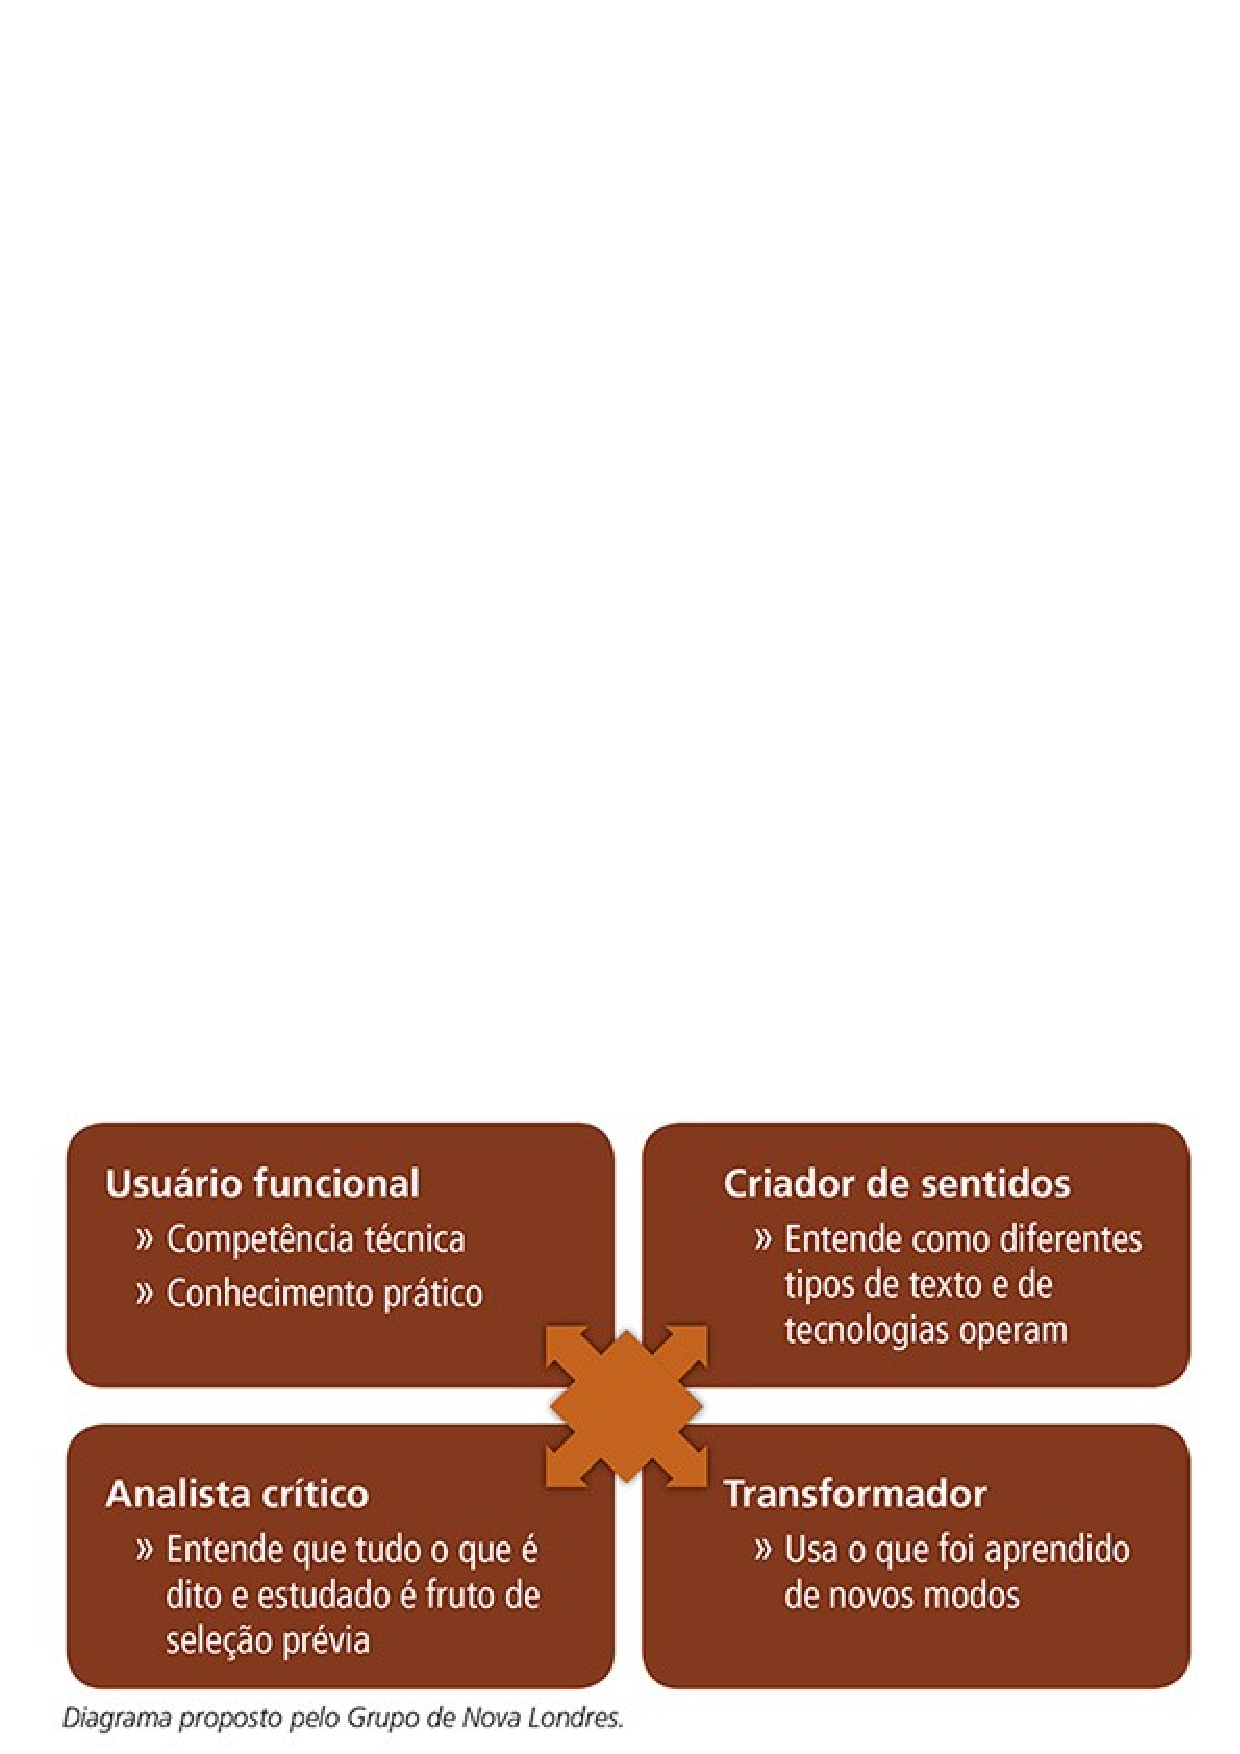
\includegraphics[width=\textwidth]{figure01.png}  
\caption{Somatório e percentual das visualizações dos vídeos integrantes da amostragem por canal.}\label{fig01}
\source{Elaboração própria (2021).}
\end{minipage}
\end{figure}

Ao se contabilizar o total de visualizações dos vídeos selecionados por
canal, observou-se que os vídeos mais populares são os que versam sobre
crimes reais (\emph{true crime}). Nesse gênero literário, os três vídeos
do canal ``Bel Rodrigues'', apesar de postados recentemente, em 2018 e
em 2019, são os mais visualizados, com 6.041.851 (44\%) visualizações. A
segunda posição, com 3.433.155 (25\%) visualizações, é dos três vídeos
do canal ``Ler até amanhecer'', postados em 2020. O conteúdo com menor
visualização foi o de ``Melina Souza'', postado em 2013, 2014 e 2017,
com 284.043 (2\%) visualizações. O canal ``Vá ler um livro'', cujos três
vídeos mais acessados são exclusivos de literatura brasileira para as
seleções que conferem acesso ao Ensino Superior, contou com 845.782
(6\%) visualizações.

Além disso, na \Cref{fig02}, demonstra-se o quantitativo de \emph{likes}
(gostei) e de \emph{dislikes }(não gostei), tendo por base o total de
visualizações alcançado pelos três vídeos agrupados por canal. De cima
para baixo, no topo das colunas, está inscrito o total de visualizações
obtido pelos vídeos examinados. As avaliações dos espectadores,
``gostei'', estão inscritas no centro, pouco acima das bases das
colunas, em percentagem. Os valores percentuais, na parte mais inferior,
à direita das colunas, refletem o julgamento ``não gostei''.

% FIGURA 2
\begin{figure}[h!]
\centering
\begin{minipage}{.75\textwidth}
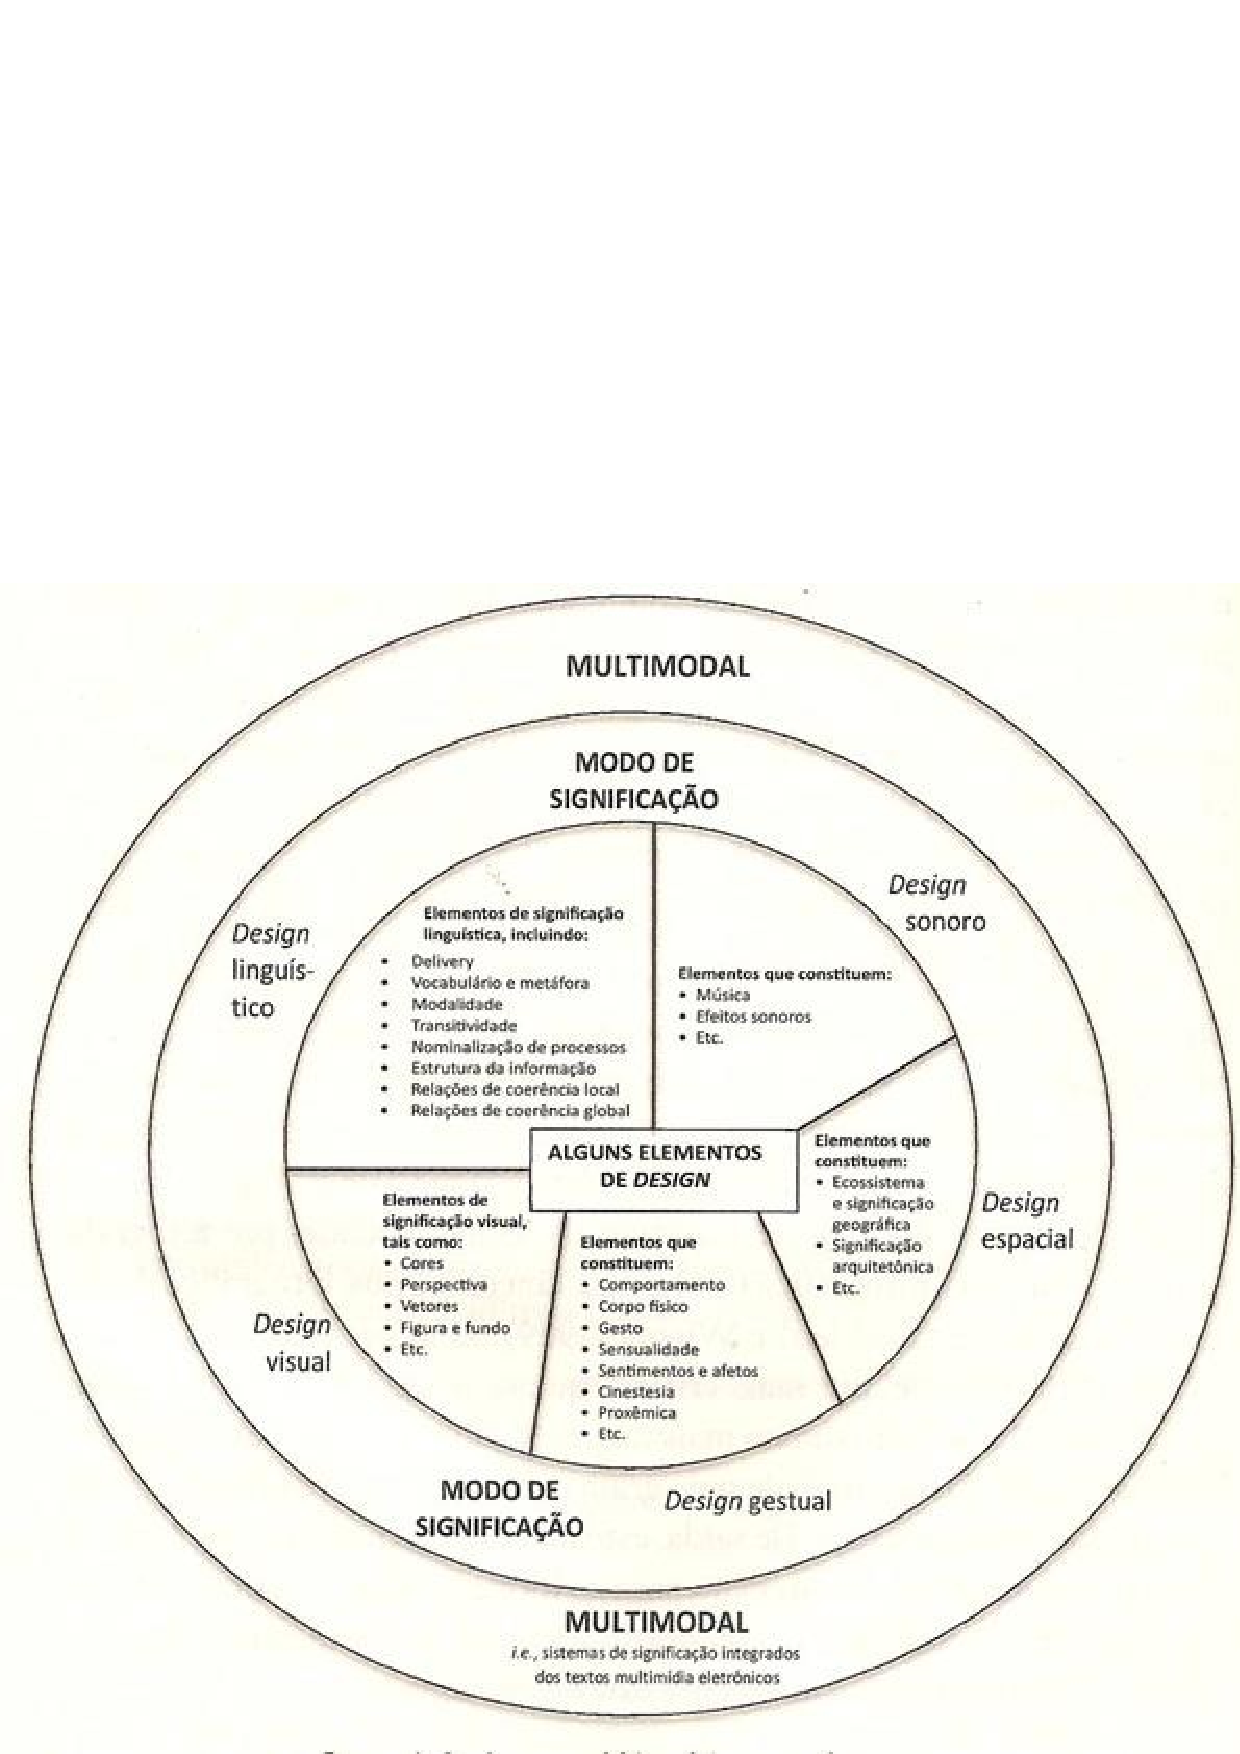
\includegraphics[width=\textwidth]{figure02.png}  
\caption{Total de visualizações e avaliações “gostei” e “não gostei”.}\label{fig02}
\source{Elaboração própria (2021).}
\end{minipage}
\end{figure}

Ainda na \Cref{fig02}, observa-se que os vídeos mais acessados, do
canal ``Bel Rodrigues'', com 6.041.851 visualizações, obtiveram 7,96\%
de \emph{likes} e 0,06\% de \emph{dislikes}, sendo classificados pelos
espectadores na terceira colocação da avaliação ``gostei'',
ultrapassados por canais com menos visualizações, a saber, ``Ler até
amanhecer'' (3.433.155 visualizações e 8,3\% gostei) e ``Ler antes de
morrer'' (1.623.270 visualizações e 8,44\% gostei). Apesar disso, em
todos os canais, poucas são as avaliações ``não gostei'', cuja soma
corresponde a somente 1\% do total das visualizações.

\section{Discussão}\label{sec-dis}
Este estudo, ao revelar que os seis canais qualificados para análise
foram criados por mulheres e que, em conjunto, reúnem 2.910.000
seguidores, 3.744 vídeos e 208.700.606 visualizações, sugere o
protagonismo delas na comunidade \emph{booktuber} brasileira.\textbf{
}Esse achado se assemelha ao dos estudos espanhóis de \textcite{Tomasena2021}, %Tomasena (2021),
que analisou a distribuição de 464 canais \emph{booktubers} de língua
espanhola em vários países, em que 62\% são conduzidos por mulheres e
32,9\% por homens\footnote{ Uma pequena parte dos 464 canais é
  administrada por bibliotecas, escolas e coletivos \cite{Tomasena2021}. % (TOMASENA, 2021).
},
e de \textcite{GarcaRoca2020}, %García-Roca (2020), 
o qual evidenciou que, dentre os 100
\emph{booktubers} mais influentes na Espanha, 79,5\% são mulheres e
20,5\% homens.

Na amplitude da abrangência temática veiculada pelas \emph{booktubers}
brasileiras, para além da educação informal, a formal é favorecida,
inclusive quanto aos temas transversais, isso porque, como aludem \textcite{fialho_formacao_2021a}, o ensino-aprendizagem rompe os limites da sala de aula
presencial e permeia os ambientes informais, transformando-os em lócus
de construção e de compartilhamento do conhecimento. Ademais, na
onipresença do território virtual, a informação é instantânea, as formas
tradicionais de leitura são modificadas e a construção do saber é
expandida cada vez mais \cite{Krug2019}. %(KRUG, 2019).

\textcite{Ferreira2018} %Ferreira e Santos (2018) 
indicam que, apesar de a escola ser a
instituição oficial do letramento, a competência para a leitura é
influenciada pelos recursos tecnológicos e pela internet, pois eles
ampliam a sala de aula física para o meio virtual, promovem interação
social e desenvolvem a criticidade dos estudantes. À vista disso, \textcite{leite2021}, %Leite (2021), 
com maestria didática, apresenta as escolas literárias,
esclarece as figuras de linguagem e resenha as obras indicadas para os
exames de acesso ao Ensino Superior no Brasil. Já \textcite{rodrigues2021} %B. Rodrigues (2021)
direciona as exposições sobre livros baseados em crimes reais para
abordar \emph{bullying} nas escolas, depressão, pensamentos suicidas,
abuso sexual e físico em crianças e adolescentes, expondo suas
concepções críticas a respeito da maneira como o sistema judicial atuou
na condução dos crimes veiculados nas obras narradas.

Os espectadores, não necessariamente os inscritos, mas aqueles que
acessam os canais, interagem com as \emph{booktubers} de duas formas:
pelos comentários e pelos \emph{links} e \emph{dislikes}. O
estudo permitiu alcançar que existe um canal de interação aberto por
todas as seis \emph{booktubers}, pois
se relacionam com os seguidores por
intermédio de fecundos comentários sobre o conteúdo propagado,
fomentando, inclusive, a comunicação entre espectadores, que também se
comunicam uns com os outros nesse espaço. Tais evidências reportam ao
estudo de \textcite{VizcanoVerd2019} %Vizcaíno-Verdú, Contreras-Pulido e Guzmán-Franco (2019) 
acerca
dos \emph{booktubers} espanhóis de alto impacto, em que, nessas
comunidades, a palavra é ampliada para os respectivos seguidores,
permitindo expandir e aprofundar novas práticas produtivas do saber,
principalmente pela afinidade entre o público juvenil, que, de mero
espectador, passa a refletir a respeito do contexto literário,
interpretando-o. Essa interação, conforme entendem \textcite{oliveira2021booktubers}, %Oliveira \emph{et al. }(2021), 
com versatilidade de horários, produz a sensação de proximidade
entre \emph{booktubers} e público. Entretanto, há de considerar o
congraçamento de \textcite{Silva2021} %Silva e Gonçalves (2021) 
de que a leitura e a escrita
mediadas pelas TDICs -- letramento digital --, como meio de alcançar o
letramento literário -- leitura e escrita de diferentes textos
literários --, requisitam o acesso à internet e o domínio das
ferramentas que lhes são próprias. Contudo, por ora, em razão das
distorções locorregionais e econômicas brasileiras, ainda muito
excludentes.

A vinculação entre comunidade \emph{booktuber} e educação alude à
essencialidade da leitura para o aprendizado crítico-reflexivo
necessário à aquisição de competências formativas pelos estudantes.
\textcite{SantosDaz2021}
%Santos Díaz, Juárez Calvillo e Trigo Ibáñez (2021) 
estudaram a motivação
para a leitura acadêmica em estudantes da Universidade de Cádiz e
descobriram que, apesar das declarações estudantis de gostar de ler, a
desmotivação para essa prática predomina. Então, indicaram que os textos
literários correspondem a 29,87\% e os acadêmicos a 1,95\% das leituras
efetuadas pelos sujeitos daquela amostragem. Ao se cotejar o estudo de
Cádiz com a pesquisa em relato, certifica-se a simetria entre ambos,
porque os vídeos dos canais ``Ler antes de morrer'' \cite{lubrano2021} %(LUBRANO, 2021) 
e ``Vá ler um livro'' \cite{leite2021} %(LEITE, 2021) 
voltados à escolarização, que abordam
os clássicos da literatura nacional e internacional e as escolas
literárias brasileiras, em conjunto, corresponderam a 18\% das
visualizações, possivelmente um indicador do minguado interesse por essa
temática.

Chamou a atenção, contudo, o conteúdo dos dois canais mais acessados,
``Bel Rodrigues'' (6.041.851 visualizações) e ``Ler até amanhecer''
(3.433.155 visualizações), por se referirem a crimes reais ocorridos no
Brasil e em outros países, quando os seis vídeos averiguados reuniram o
expressivo número de 9.475.006 (69\%) visualizações \cite{rodrigues2021,rodriguesjoici2021}, 
%(RODRIGUES, B., 2021; RODRIGUES, J., 2021), 
fazendo aflorar a inquietude a respeito da
razão da predileção dos leitores por tal gênero. Para esclarecer,
\textcite{Browder2010} %Browder (2010) 
leciona que as obras literárias sobre crimes verdadeiros
pertencem ao gênero híbrido, denominando-se \emph{true crime}. Dentre
suas características, a escrita é próxima à ficção policial e à
romântica, mas com dados reais documentais. Além disso, exercem imensa
atratividade sobre os leitores, que se envolvem, muitas vezes,
profundamente com a leitura e se posicionam em relação às vítimas, aos
criminosos e aos policiais, investigadores e outros agentes, numa
relação complexa ou mesmo contraditória.

Malgrado a constatação de canais com \emph{playlists} heterogêneas, a
aquiescência à leitura é o principal escopo das \emph{booktubers}
investigadas, as quais transitam por gêneros variados sem deixar escoar
a oportunidade para se posicionarem a respeito dos enredos e de outras
questões correlatas. Provam-se essas menções por \textcite{feltrin2021}, %Feltrin (2021), 
que critica veementemente a trilogia romântica erótica britânica escrita por
E. L. James, sobretudo o perfil sadomasoquista do protagonista e a
maneira como a protagonista transforma-se no exercício da sexualidade.
Sinaliza a \emph{booktuber} que o grande interesse por obras desse tipo
se dá em razão da curiosidade e do trabalho midiático atrativo dos
leitores. Outro julgamento feito por Tatiana Feltrin, a partir do
paradigma da coleção Harry Potter, é no tocante aos problemas de
tradução da língua estrangeira para o português e ao alto custo das
obras, que se antagonizam à baixa qualidade do material utilizado na
confecção dos livros pelas editoras brasileiras. Inclusive, compara
preço e qualidade das versões estrangeiras e nacionais. Além disso, ante
a existência de filmes baseados em livros, declara sua predileção pelos
livros e denuncia que, na maioria das vezes, o cinema falha em retratar
a essência dos livros.

De maneira geral, a linguagem utilizada nas vídeo-resenhas é fluente e
bastante diversificada. Algumas \emph{booktubers} utilizam termos
coloquiais, outras intercalam expressões em inglês, presumivelmente na
intenção de adequar a oralidade à compreensão do público e aos termos
próprios dos \emph{videoblogueiros} literários, sendo que a
multimodalidade é proeminente nessas apresentações. Com efeito, Britto e
Silva (2019) cientificam que a vídeo-resenha é um gênero emergente e
multimodal complementar à prática docente que possui estrutura
composicional de resenha e recursos estilísticos próprios de vídeos,
cujos autores utilizam-se de imagens e de reforço linguístico, como
gesto, entonação, ênfase e ritmo de fala, para aumentar a capacidade
cognitiva e interpretativa do público. Em conformidade, \textcite{Pena2020} %Pena (2020)
assevera, na multimodalidade, que tais combinações na mesma mensagem
favorecem o entendimento em confluência com o contexto situacional,
sociocultural, da qual emergiu. Concorda-se com a opinião de \textcite{oliveira2021booktubers} %Oliveira \emph{et al. }(2021) 
quando inferem que a linguagem menos formal, livre
e divertida pode amenizar a visão engessada da biblioteca diante da
sociedade e produzir a compreensão de que a prática da leitura é
agradável. Concordam também \textcite{RomeroOliva2021}, %Romero Oliva, Heredia Ponce e Rivera Jurado (2021), 
pois, para propiciar a compreensão e o prazer pela leitura de
obras clássicas em populações como a infantil, é necessário utilizar
metodologias inovadoras com as adaptações compatíveis com as
especificidades dos alunos.

As \emph{booktubers} orientam como aderir à leitura e como otimizá-la
mediante cautela na escolha da edição e da tradução da obra de
interesse, principalmente dos clássicos originários em língua
estrangeira. Em se tratando da literatura brasileira mais antiga, que
contém linguagem mais erudita, propõem compreender as palavras
desconhecidas na totalidade do texto e com o contexto, sem pausas para
consultar dicionários, evitando, portanto, interferir na continuidade do
ato. Para construir mentalmente a imagem do que se lê, aconselham o
apoio dos recursos existentes na internet sobre a época, a geografia e a
cultura relacionados ao tempo e ao espaço referidos na obra. Para não
``se perder'' no livro, destacam a importância de atentar para a
integralidade da obra, ler prefácios, introduções, comentários, orelhas
e outras informações antes de iniciar a leitura dos capítulos \cite{lubrano2021}. % (LUBRANO, 2021).

Depreende-se dos vídeos sondados que as \emph{booktubers} ultrapassam as
fronteiras das vídeo-resenhas e transitam pelos demais elementos que
compõem o âmbito literário. Mesmo se autoavaliando como não
especialistas, lançam-se a avaliar produtos vinculados à leitura, como é
o caso dos equipamentos leitores digitais \cite{feltrin2021}, % (FELTRIN, 2021), 
e realizam \emph{bookshelfs}, apresentando suas estantes de livros \cite{souza2021}. 
% (SOUZA, 2021).

Por fim, todos os canais remetem a \emph{links} para a aquisição dos
livros apresentados. Igualmente, \textcite{Tomasena2021} %Tomasena (2021) 
informa que os
\emph{booktubers} são prescritores de livros e grandes aliados das
editoras, por isso contemplam o interesse comercial. Mas, como conclui o
estudo de \textcite{GarcaRoca2020}, %García-Roca (2020), 
a partir da análise dos mais notáveis
\emph{booktubers} espanhóis, eles são motivadores de consumo confiáveis,
alinhados à educação formal e à formação literária.

\section{Considerações finais}\label{sec-con}
O presente estudo foi concebido a partir da inquietação acerca do
conteúdo difundido pelos \emph{booktubers} brasileiros mais populares,
que agregam 100 mil ou mais seguidores. Logo, objetivou-se investigar os
principais canais literários e o conteúdo veiculado pelos
\emph{booktubers} mais influentes do Brasil. Para atender a tal escopo,
empreendeu-se uma pesquisa quantiqualitativa que investigou seis canais
e 18 vídeos disponibilizados abertamente no YouTube.

Evidenciou-se que todos os canais que atenderam aos critérios de
inclusão foram criados por mulheres brancas, no período de setembro de
2007 a agosto de 2018, os quais, em conjunto, congregam 2.910.000
inscritos, com uma média anual de 624 vídeos e 34.783.434 visualizações.
Não obstante o expressivo número de visualizações e de seguidores, o
estudo não permitiu afirmar se efetivamente os conteúdos foram
alcançados por completo, porque visualizações diferem de assistir
inteiramente aos vídeos. Todavia, indicam o significativo e crescente
interesse do público pelas obras veiculadas: livros do gênero \emph{true
crime}, romance, aventura, fantasia, ficção, incluindo clássicos da
literatura nacional e internacional. Apesar de a mediação da leitura ser
o principal mote das \emph{booktubers}, alguns canais oferecem
vídeos sobre outras temáticas: viagens, intercâmbios, compras e outros.

Em termos quantitativos, o maior número de visualizações, 9.474.905
(69\%), foi dos seis vídeos sobre livros integrantes do gênero
\emph{true crime}. Por outro lado, três vídeos literários de livros
empregados nos concursos de acesso ao Ensino Superior no Brasil
obtiveram 6\% das visualizações e três vídeos acerca de orientações para
aderir à leitura e de sínteses sobre clássicos da literatura brasileira
e estrangeira alcançaram 12\%. As narrativas, na perspectiva multimodal,
perpassam por outros aspectos vinculados à leitura, a exemplo da
indicação de marcas de leitores digitais e das recomendações de compras
das obras apresentadas.

Além disso, destaca-se que este estudo proporcionou conhecer a produção
difundida por seis \emph{booktubers} brasileiras, influentes em
correspondência ao interesse do público pelos respectivos canais e pelo
conteúdo divulgado, conforme expresso no quantitativo de seguidores e de
visualizações que os canais e vídeos aglutinam. Ademais, tornou-se
possível afirmar que os livros literários de crime baseados em fatos são
os que mais despertam a atenção do público jovem.

Depreende-se que a comunidade \emph{booktuber} exerce relevante papel à
educação informal e formal, mas, considerando que o acesso à plataforma
YouTube se dá mediante as TDICs, o alcance daqueles alijados da inclusão
digital não é equânime. Dessa maneira, ainda que os canais estimulem a
leitura por despertar a curiosidade dos seguidores e por possibilitar a
participação nos debates, ante a severa desigualdade social, muitos
brasileiros sequer possuem condições econômicas para dispor de acesso à
internet e aos equipamentos digitais e de compra dos livros indicados.

Esta pesquisa também permite lançar luz às inovadoras maneiras de
estimular a leitura, a exemplo dos canais de \emph{booktubers}, por
vezes pouco valorizadas ou até mesmo desconhecidas pelos professores
brasileiros. Todavia, a ampla aderência a esses canais permite asseverar
não apenas a necessidade de políticas públicas para fomentar maior
justiça social e acesso às TDICs e aos livros à população, como também a
urgência de formação de professores para explorar e trabalhar as TDICs
em prol de uma educação mais atrativa e imbricada com as demandas de uma
juventude cada vez mais digital e conectada, sabendo-se que ainda são
escassas as pesquisas sobre essa temática no Brasil.

Uma das limitações do estudo é a possibilidade de outros canais
literários influentes não terem sido abarcados pelos critérios de busca.
Com efeito, o estudo permitiu refletir acerca da abundância do universo
informacional em torno do objetivo de investigação. Confia-se, então, na
relevância da pesquisa por trazer ao debate um tema de interesse para a
sociedade e para os pesquisadores dedicados a compreender as novas
nuanças do meio educacional e literário.

Para estudos futuros, sugere-se analisar o conteúdo dos comentários
postados pelos canais com a finalidade de: entender a percepção do
público a respeito dos canais e suas interações; monitorar a
popularidade desses canais; ou para repisar a busca em um lapso temporal
mais adiante, compreendendo a ampliação ou a diminuição do movimento de
incentivo à leitura intermediado por \emph{booktubers}.





\printbibliography\label{sec-bib}
% if the text is not in Portuguese, it might be necessary to use the code below instead to print the correct ABNT abbreviations [s.n.], [s.l.]
%\begin{portuguese}
%\printbibliography[title={Bibliography}]
%\end{portuguese}


%full list: conceptualization,datacuration,formalanalysis,funding,investigation,methodology,projadm,resources,software,supervision,validation,visualization,writing,review
\begin{contributors}[sec-contributors]
\authorcontribution{Lia Machado Fiuza Fialho}[projadm,supervision,validation,writing,review]
\authorcontribution{Vanusa Nascimento Sabino Neves}[conceptualization,datacuration,methodology,formalanalysis,writing]
\end{contributors}


\end{document}

